\chapter{Background}

\newtheorem{defi}{Definition} % Start new Definetion numbering

\section{Phylogeny}
\subsection{Overview}

The branching pattern of ancestor/descendant relationships among species or
their parts (e.g., genes) is a phylogeny. Researchers attempt to estimate these 
historical relationships by examining character evolution using a tree - a mathematical
structure used to model the actual evolutionary history of species or their parts.
These inferred trees (historical branching relationships) can be represented as 
cladograms, where branch lengths are arbitrary and only the branching order is significant,
or as phylograms, where the branch lengths are proportional to the amount of evolutionary 
change along the branch.

Phylogenies were historically used to classify organisms into natural evolutionary
groups based on these ancestor/descendant relationships. Indeed, great effort is
currently being spent on estimating the Tree of Life to quantify the biodiversity of
our planet. However, phylogenies have also spread in use as the utility of the
evolutionary framework for numerous other disciplines becomes increasingly obvious. 
For example, phylogenies are now being extensively used in the biomedical sciences 
including developmental biology, genomic biology, infectious disease, virology,
and human genetics \cite{jumpstarting}.

\subsection{Phylogeny Tree}
Since this thesis is about phylogenetic trees, it is therefore 
appropriate to start by defining a tree \cite{alkim}. 
Trees can be classified as unrooted or rooted phylogenetic trees. An 
unrooted phylogenetic tree or just unrooted tree is an acyclic connected 
graph having no internal vertices of degree two and every leaf having 
different label. The leaves are vertices of degree one \ref{img:sample1}.

\begin{figure}[!htbp] 
  \center
  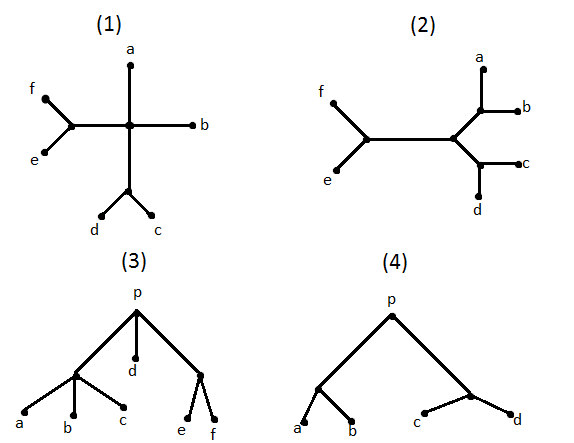
\includegraphics{tree1}
  \caption[w]{Four examples of phylogenetic trees. (1) and (2) are unrooted. (3) and 
(4) are rooted. (2) and (4) are binary. } 
  \label{img:sample1}  
\end{figure}

A rooted tree on tree, on the other hand, is similar to an unrooted 
tree, except it has one internal vertex of degree two, which is called the 
root. The internal vertices of unrooted/rooted (except the root) trees can 
have degree three or greater. For example a binary phylogenetic tree, is a 
tree having all internal vertices of degree three. Again the only exception is 
the root, which has degree two \ref{img:sample2}. In a fully resolved binary 
phylogenetic tree with n leaf nodes there are n-1 internal nodes. 

\begin{figure}[!htbp] 
  \center
  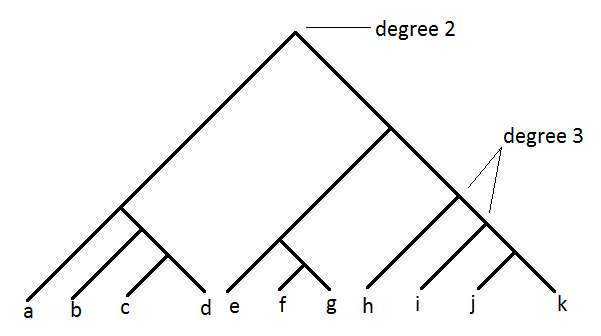
\includegraphics{tree2}
  \caption[w]{In a binary tree each internal node has degree three with the 
exception of the root which has degree two.} 
  \label{img:sample2}  
\end{figure}

The leaves of the tree represent species. For example let L(T) be the 
set of leaves for tree T. If T the set of trees, then we can say that L(T) is the 
union of the leaf sets of the trees in T. 

In a rooted tree we say that a vertex a is an ancestor of a vertex b, if 
the path from b to the root passes through a. We can also say that b is the 
descendant of a.  

The vertices adjacent to a vertex that are descendants of the vertex 
are called the children of the vertex, and the adjacent vertex that is an 
ancestor is called the parent of that vertex. Sometimes the internal 
vertices of a phylogenetic tree are labelled (section Nested Taxa). 

Rooted phylogenetic trees can be displayed with a vertical axis 
representing the time each branching point occurred. These diagrams are 
called dendograms \ref{img:sample3}. 

\begin{figure}[!htbp] 
  \center
  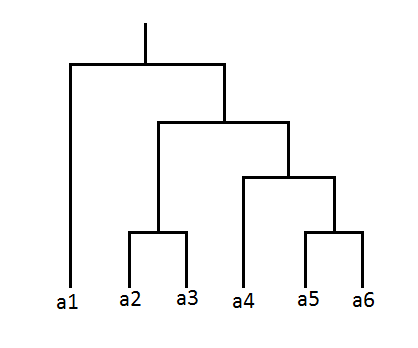
\includegraphics{tree3}
  \caption[w]{An example of dendogram.} 
  \label{img:sample3}  
\end{figure}

Let T be a rooted tree and choose a vertex v in T. If we remove the 
edge between v and the parent of v, say p, we get two connected 
subgraphs. Then let v be the root of the subgraphs containing v, then this 
is called the subtree of T rooted at v. Briefly a subtree T' is a tree whose 
vertices and edges form the subsets of the vertices and edges of a given 
tree T. An example of a subtree is shown in \ref{img:sample4}.

\begin{figure}[!htbp] 
  \center
  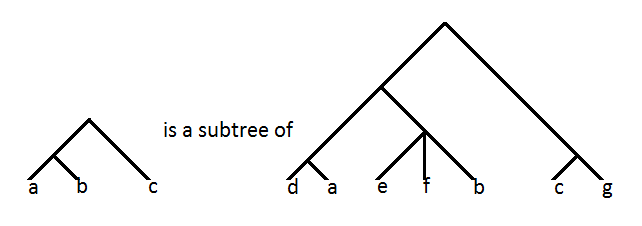
\includegraphics{tree4}
  \caption[w]{Example of a subtree.} 
  \label{img:sample4}  
\end{figure} 

For every three leaves a, b, c there are four possible rooted trees 
with leaf set a, b, c.  

The binary rooted trees on three leaves are called rooted triples and 
((ab)c) (or ab|c) denotes the rooted triple with a pair of leaves a, b 
connected to a third leaf c via the root (\ref{img:sample5}). For a rooted triple 
((ab)c) to fit a rooted tree T, the path from a to b does not share any 
vertices with the path from c to the root. Briefly a rooted triple is a tree 
with three leaves and two internal vertices. 

\begin{figure}[!htbp] 
  \center
  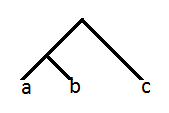
\includegraphics{tree5}
  \caption[w]{ A binary rooted triple ((ab)c).} 
  \label{img:sample5}  
\end{figure} 

Non-binary rooted trees with three leaves are called fan triples. We 
call a fan with k leaves a k-fan. 

% Also it has many useful features such as making presentations, 
% importing from most popular file formats as well as exporting 
% to these formats.

\section{Estimate colculations algorithms}
Abstract - Most of the advanced data processing and analysis technologies 
designed for solving domain-specific problems employ the automation and 
optimization techniques of decision-making based on 'real' (incomplete, 
indirect, heterogeneous, inconsistent, erroneous, etc.) information. 
The methods of mathematical theory of pattern recognition play an important role here. 
To carry out image recognition, we need an image representation that 
corresponds to the requirements of the efficient recognition algorithm chosen 
for the task. A vast majority of the efficient image recognition algorithms 
only work with image descriptions or models. To completely use the information 
contained in images, it is necessary to overcome the principal discrepancy between 
the nature of images and the data-extraction techniques based on symbol models of 
images. Thus, there is a practical need for an efficient recognition algorithm that 
directly deals with images and their fragments. More-over, the algorithm should 
provide the possibility of posing and solving the problem of choosing the best
recognition algorithm. This class of algorithms - algorithms of estimate calculations 
based on 2D information (2D-AEC)- was defined by I. Gurevich as a special type of 
the classical model of the recognition algorithms based on estimate calculations 
(AEC) introduced by Yu. Zhuravlev. Generally, the AEC model can cope with the spatial 
(2D) image structure. The principal feature of the 2D-AEC is the use of the proximity 
of objects in spatial support sets, i.e., in images and their fragments. The range 
of the problems of 2D-AEC includes the enumeration and investigation of spatial 
support sets as well as definition of the subclasses of algorithms (corre- sponding 
to the types of the support sets) which allow one to produce efficient formulas that 
model the work of the algorithms. In this work, we find these formulas for the particular 
subclass of 2D-AEC - algorithms of estimate calculations with rectangular support sets.
\subsection{Overview}

%Unit testing \label{1st_ex} first introduced by Kent Beck
%in the Smalltalk language and then the concept has 
%been adapted to other languages.  

Most of the current data technologies for information processing and analysis designed 
to solve domain-specific content-driven problems employ the automation and optimization 
techniques of operative decision-making based on 'real' (incomplete, indirect, heterogeneous,
inconsistent, erroneous, etc.) information. These information technologies are widely 
used in medical and technical diagnoses, nondestructive testing, ecological monitoring,
natural disaster and emergency forecasting (like technogenic catastrophes, earthquakes, 
fioods, forest fires), informa- tion and copyright protection, security systems, 
scientific research automation, smart weapons, remote earth sensing, criminal law, 
and control. The methods of mathe- matical theory of pattern recognition are the basic 
tools for solving all of these problems. In most cases, when initial data are completely 
or partly represented as images, it is necessary to use the methods of analysis and 
estimation of information represented by images. 

A vast majority of problems which arise 
during image analysis are, naturally, pattern recognition problems. At the same time, 
the problems of image recognition  per se  are formulated and solved much more seldom 
than is required by practical needs. The reasons are quite evident. At the informational 
level, the main difficulties are connected to the following two problems: 
(i) image description (modeling) and (ii) development and optimization of the choice of 
mathematical methods for image transformations. The solution to the image recognition 
problem implies that (i) there is an image representation and an efficient recognition 
algorithm and (ii) this representation corresponds to the requirements which the 
algorithm imposes on the initial data. Generally, in recognition problems, 
there are only two ways of data representation: (i) as direct spatial information 
(e.g., by pixels or a local neighborhood of the second order that consists of pixel 
arrays) and (ii) as a system of objects and relations extracted in images. 
Before applying a recognition algorithm, it is neces- sary to present initial 
data in the form convenient for recognition. In the first case, a recognition 
algorithm should allow the image itself or its fragments to be processed; here, 
the procedures of transforming the initial data in the form convenient for recognition 
are reduced to choosing the shape of the fragments whereby the recognized object 
is matched to the template, to fragmenting the image, etc.

In the second case, the procedures of transforming the initial data in the form 
convenient for recognition should yield a mathematical model of an image. 
This model should refiect the inner structure and content of the image as an 
outcome of operations that construct the image from the subimages and other 
objects of simpler nature, i.e., from the primitives and objects extracted in the 
image at different stages of processing. During image recognition, one should use 
information refiecting the way of pattern formation, i.e., of the image as a whole, 
and of the objects presented in the image.  

Three types of information characterize an image: (i) identifiable objects with a 
well-defined structure; (ii) identifiable objects with an ill-defined structure; 
and (iii) nonidentifiable objects. To allow for an image structure means to extract 
subimages (objects) in an image, to define the possible elementary level for them, 
and to define the relations between these objects and elements. As a result, 
the hierarchical structural information of an image may be explicitly presented and 
utilized. An image is described by a system of objects, each object is described by 
simpler objects, etc. The structural information can be introduced into recognition 
process in two ways. 

First, according to classical pattern recognition theory, 
we can use the list of features as a main formalization principle and 

(a) two 
types of features are introduced in the description; they refiect a two-dimensional 
character of the object to be recognized: 

-characteristics which refiect the properties of some local image fragment 
(the distribution of pixel values in this fragment, the presence or 
absence of a certain geometrical object in this fragment, the type of 
the object's shape, etc.); 

-characteristics of relations of separate objects and features; 

(b) the weights are assigned to the features, which indicate the degree 
of their importance for image description; 

(c) separate features are combined into a system of features and treated 
as a single feature. 

\subsection{General characterustics of the AEC class}

The model of algorithms based on calculation of the estimates 
(AEC) was successfully used for solving many problems of pattern 
recognition. The model describes the structure of recognition 
algorithm and parameters necessary for choosing particular 
algorithm in the model. In the framework of a model, the algorithms 
differ by their parameters and, therefore, by the way of their 
classification of the given objects. The results of applying the 
algorithm of a model to the test sample show the adequacy of this 
algorithm to the problem at hand. Thus, all of the algorithms 
of a given model can be supplied with a quality functional. 

The choice and/or synthesis of the algorithm, extreme according 
to the quality functional, presents the main problem in implementing 
AEC in practice. This problem is closely connected to the reduction 
of the computational complexity of AEC. The algorithms of acceptable 
computational complexity are based on efficient formulas which model 
the algorithm`s performance; these are formulas for calculating 
proximity estimates of objects under recognition and precedents. 
The complexity of formulas for estimate calculations substantially 
depends on the AEC parameters, such as the system of support 
sets and the type of proximity function. A recognition algorithm 
uses a system of support sets as a system of feature subsets 
for matching object descriptions. A proximity function defines 
whether the matched objects are 'close'. 

By now, the most comprehensive study concerned the problems 
of deriving efficient formulas for AEC in the case where all 
available objects are described by the one-dimensional feature 
vectors and the support sets encode the parts of these one-dimensional 
descriptions. This problem was solved for the main subclasses of AEC in.

When the efficient formulas for estimate calculations are constructed, 
the optimal (for the given model) algorithm can be chosen by 
one of the classical optimi- zation techniques or by modifying 
these techniques. A lot of research was devoted to this problem.
  
Although the efficient formulas are constructed almost for every 
AEC model of practical interest, the problem of constructing such 
formulas in the case where the objects are images, object 
descriptions are 2D matrices, and support sets are spatial (2D) 
objects still needs to be solved. As was noted above, the AEC 
class was specialized to operate with 2D object descriptions 
called a class of algorithms of estimate calculation from 
two-dimensional information (2D-AEC). Note that, by now, 
the efficient formulas are con- structed for one 2D-AEC subclass 
only: for a subclass with a square as a generative element of the 
system of support sets.

Here, we propose the method for constructing the efficient algorithms 
for the 2D-AEC subclass with two-dimensional support sets generated 
by a rectangle. The idea underlying this procedure consists in 
transforming the rectangle with the sides  $R_1*R_2$  into 
the unit square by compressing the plane along the one side  $R_1$  
times and along the other  $R_2$  times. 

Let us recall the basic objects and properties of the AEC model 
Generally, a recognition algo- rithm contains a recognizing operator and a 
decision rule. In AEC, a recognizing operator converts a standard 
description of object $S$ , subject to recognition into a 
set of numerical estimates $(\Gamma_1(S),\Gamma_2(S),\ldots,\Gamma_l(S))$,
where $l$ is a number of clases.  A decision rule helps us to 
construct the information vector $(\alpha_1,\alpha_2,\ldots,\alpha_l)$,
$a_j\in\{0,1,\Delta\}$, from this set.  Here, $\alpha_j  = 0$ if an algorithm does not
assign object  $S$ to $j$th class;  and  $\alpha_j  =  \Delta$ 
if an algorithm cannot classify object  $S$ . To define a recognizing operator, 
it is necessary to assign a system of support sets, proximity function, 
feature weights, and precedent weights. Let us consider these parameters in detail.  

1. System of support sets. 

A system of support sets is a totality of nonempty subsets of the feature set  
$N  = \{1,2,\ldots,n\};$ the object is described by the values of these features. 
A system of support sets is denoted by  $\Omega_A$. 
Below, we list the examples of support sets.

1.1. $\Omega_A  = 2^N;$ i.e., a system of support sets is a class of all (nonempty) 
subsets of feature set  $N$.
 
1.2.  $\Omega_A=\{\Omega|\Omega\subseteq N,|\Omega|=k\}$, where  $k$  is an integer and $1\leq k\leq n;$ 
i.e., a system of support sets consists of all of the subsets of the set  $N$  which have 
a predefined power  k , e.g.,  $\Omega_A={{1},{2},\ldots,{n}}$ for  $k=1$ and $\Omega_A=\{N\}$ for  $k=n$. 
The following relation connects the systems of support sets of 1.1 and 1.2:

$$
2^N=\bigcup_{k=1}^n\{\Omega | \Omega \subseteq N, | \Omega | = k\}.
$$

1.3. $\Omega_A=\{\Omega|\Omega\subseteq N,|\Omega|\leq k\}$, where  $k$  is an integer
and $1\leq k\leq n;$ i.e.,  $\Omega_A$ consists of all of the subsets of the
set $N$ which have a power no more than the predefined one. 

1.4. $\Omega_A=\{\Omega|\Omega\subseteq N,|\Omega|\subseteq \{k_1,k_2,\ldots,k_u\}\}$, where 
$k_1,k_2,\ldots,k_u$  are integers and $1\leq ki \leq n, i=TODO$. 

Any support set $\Omega$ 
can be encoded by the binary vector $\tilde{\omega}$ of the length $n$ in the following way: 
the ith coordinate $\tilde{\omega}$ is equal to one if and only if the $i$th feature is contained 
in $\Omega$. The thus-constructed $\tilde{\omega}$ vector is called a characteristic vector 
of the support set $\Omega$. It is obvious that a set $\Omega$ and its characteristic 
vector $\tilde{\omega}$ are connected by a one-to-one correspondence.

Sometimes, it is convenient to consider a system of support sets as a set of characteristic 
vectors that encode the support sets of the algorithm. In those cases, we consider $\Omega_A$ 
to be a set of vertices $\{\tilde{\omega}\}$ of $n$-dimensional Boolean cube $E^n$. 

As usual, we denote the norm (weight) of the binary vector $\|\{\tilde{\omega}\}\|$ equal to 
the number of its unitary coordinates by $\{\tilde{\omega}\}$. The set of all binary vectors 
of the weight $k$ is called the $k$th layer of the Boolean cube and denoted by $E_n^k$.

We call the Boolean function $f_A(\tilde{\omega})$ a characteristic function of the system of support 
sets $\Omega_A$ if $f_A(\tilde{\omega})=1\Leftrightarrow \in \Omega_A$. Obviously, a system of support 
sets of the algorithm is unambiguously described by its characteristic function. 

The characteristic function of a system of support sets of (1.1)-type vanishes only if all its 
variables vanish.

For a system of support sets of (1.2)-type, the characteristic function is 
equal to unity in the whole layer of Boolean cube and only there.

For a system of support sets of (1.3)-type, the characteristic function is equal to 
unity in the whole first, second, \ldots, $k$th layers of Boolean cube and only there.   

2. Proximity function.

Let $I(S) = (a_1, a_2, \ldots, a_n)$ be a standard (feature) description of 
object $S, \Omega = \{i_1, i_2,\ldots, i_k\}$, and let  be a characteristic 
vector $\Omega$. We denote a subdescription of the object $S$ represented in 
the form $(a_{i_1}, a_{i_2} ,\ldots,a_{i_k})$ by the symbols 
$\tilde{\omega} I(S)$ or $\tilde{\omega}(S)$.

The proximity function $B_{\tilde{\omega}}(S, S')$ depends on $\tilde{\omega}$-subdescriptions 
of objects $S, S'$ and takes two values: 0 if the objects are not close and 1 otherwise. 

Most often, the following proximity functions are considered:

2.1
\begin{equation}
B_{\tilde{\omega}}(S, S') = \left\{ 
  \begin{array}{l l}
    1, \tilde{\omega}S = \tilde{\omega}S' \\
    0, \tilde{\omega}S \neq \tilde{\omega}S'
  \end{array} \right.
\end{equation}

2.2. Let the metric (or semimetric) $\rho_i(x, y), i = \bar{1,n}$, be defined on the 
range of definition of the $i$th feature. 
Let $\tilde{\omega}S=(a_{i_1}, a_{i_2}, \ldots, a_{i_k}), \tilde{\omega}S' = (b_{i_1}, b_{i_1}, \ldots, b_{i_1})$,
and the quantities $\varepsilon_i \geq 0, i = \bar{1, n}, \varepsilon \geq 0$, where $\varepsilon$ 
is integer, be set. Consider a system of inequalities
\begin{equation}
	\rho_{i_1}(a_{i_1}, b_{i_1}) \leq \varepsilon_{i_1},
	\rho_{i_2}(a_{i_2}, b_{i_2}) \leq \varepsilon_{i_2},
	\ldots,
	\rho_{i_k}(a_{i_k}, b_{i_k}) \leq \varepsilon_{i_k}	
\end{equation}
and denote the number of unsatisfied inequalities in this system by $\gamma$. Then,
\begin{equation}
B_{\tilde{\omega}}(S,S') = \left\{ 
  \begin{array}{l l}
    1, \gamma \leq \varepsilon \\
    0, \gamma > \varepsilon
  \end{array} \right.
\end{equation}

The parameters of this function are the vector 
$\varepsilon = (\varepsilon_1, \varepsilon_2, \ldots, \varepsilon_n)$ 
and the quantity $\varepsilon$ (maximally admissible number of unsatisfied 
inequalities in system (1.2)). If $\varepsilon_i = 0, i = \bar{1,n}$, and $\varepsilon = 0$, this 
proximity function is identically equal to the proximity 
function determined in 2.1.

2.3.  If in the conditions of the previous point, we set two 
integers $\varepsilon^1$ and $\varepsilon^2$ ($\varepsilon^1$, $\varepsilon^2$ $\geq$ 0) instead 
of $\varepsilon$, then

\begin{equation}
B_{\tilde{\omega}}(S, S') = \left\{ 
  \begin{array}{l l}
    1, \|\{\tilde{\omega}\}\| - \gamma \geq \varepsilon^1,\gamma \leq \varepsilon^2 \\
    0, \gamma > \text{otherwise}
  \end{array} \right.
\end{equation}

Vector $\varepsilon = (\varepsilon_1, \varepsilon_2, \ldots , \varepsilon_n)$ and 
quantities $\varepsilon^1$ and $\varepsilon^2$ (minimal accessible 
number of satisfied inequalities in system (1.2) and maximal accessible number 
of unsatisfied inequalities in system (1.2), respectively) are parameters of 
the function. For $\varepsilon^1 = 0$ and $\varepsilon^2 = \varepsilon$, we get the (2.2)-type proximity function.

Suppose once more that $I(S) = (a_1, a_2, \ldots, a_n)$,
$I(S') = (b_1, b_2, \ldots, b_n)$, the metric (or semimetric) $\rho_i(x, y)$
is defined in the range of definition of the ith feature, and the values $\varepsilon_i \geq 0, i = \bar{1, n}$ are set. 
The binary vector $\tilde{\delta} = \tilde{\delta}(S, S') = (\tilde{\delta}_1, \tilde{\delta}_2, \ldots, \tilde{\delta}_n)$ defined as follows: 

\begin{equation}
\delta_i = \left\{ 
  \begin{array}{l l}
    1, \rho_i(a_i,b_i) \leq \varepsilon_i \\
    0, \rho_i(a_i,b_i) > \varepsilon_i
  \end{array} \right.
\end{equation}

where $i = \bar{1,n}$, is called a characteristic vector of the proximity 
of objects $S$ and $S'$.

By using a characteristic vector of proximity, we can rewrite the expression for 
(2.2)-type proximity function as

\begin{equation}
B_{\tilde{\omega}}(S, S') = \left\{ 
  \begin{array}{l l}
    1, (\tilde{\delta'}, \tilde{\omega}) \leq \varepsilon \\
    0, (\tilde{\delta'}, \tilde{\omega}) > \varepsilon
  \end{array} \right.
\end{equation}

where $\tilde{\delta'}$ is a binary vector obtained by the coordinate-wise negation of vector 
$\tilde{\delta} $ and $(\alpha, \beta)$ is a scalar product of the vectors $\alpha$ and $\beta$ which is 
equal to the sum of their coordinatewise multiplications. 

In a similar way, for the (2.3)-type proximity function,

\begin{equation}
B_{\tilde{\omega}}(S, S') = \left\{ 
  \begin{array}{l l}
    1, (\tilde{\delta}, \tilde{\omega}) \geq \varepsilon^1, (\tilde{\delta'}, \tilde{\omega}) \geq \varepsilon^2 \\
    0, \text{otherwise}
  \end{array} \right.
\end{equation}

We can introduce vector $\tilde{\delta}(S, S')$ while ignoring the metric 
$\rho_i$ and quantities $\varepsilon_i$ in the following way:

\begin{equation}
\delta_i = \left\{ 
  \begin{array}{l l}
    1, a_i = b_i \\
    0, a_i \neq b_i
  \end{array} \right.
\end{equation}

In this case, the expression for the (2.1)-type proximity 
function can be rewritten in the following way:

\begin{equation}
B_{\tilde{\omega}}(S, S') = \left\{ 
  \begin{array}{l l}
    1, (\tilde{\delta}, \tilde{\omega}) = \|\tilde{\omega}\| \\
    0, (\tilde{\delta}, \tilde{\omega}) < \|\tilde{\omega}\|
  \end{array} \right.
\end{equation}

3. Feature weights. 

Feature weights are set by the vector 
$\textbf{p} = (p_1, p_2, \ldots, p_n), p_i > 0, i = \bar{1, n}$. 

Let ${i_1, i_2, \ldots, i_k}$ be a set of the indices of all unit 
coordinates of the characteristic vector $\tilde{\omega}$. The weight 
of the support set $\Omega$ with a characteristic vector $\tilde{\omega}$ 
is denoted by $p(\tilde{\omega});  p(\tilde{\omega}) = p_{i_1} + p_{i_2} + \ldots+ p_{i_k}$.

4. Precedent weights.

Precedent weights are defined by the vector 
$ \gamma = (\gamma_1, \gamma_2, \ldots, \gamma_{m})$, 
where $\gamma_q = \gamma(S_q)>0, q = \bar{1, m} $, and $m$ is a 
total number of precedents. This point concludes the list of 
the parameters of the recognition operator of AEC.

The estimate $\Gamma_j(S)$ of the object $S$ over the $j$th class 
is defined by the following formula:

\begin{equation}
\Gamma_i(S) = \frac{1}{K}\frac{1}{|W_j|}\sum_{S'\in W_j}\gamma(S')\sum_{\tilde{\omega}\in\Omega_A}p(\tilde{\omega})B_{\tilde{\omega}}(S, S'), j = \bar{1, l},
\end{equation}
where $K$ is a normalized coefficient and $W_j$ is a set of precedents of the $j$th class. 

Sometimes we use the formulas to assess an esti- mate $\Gamma_j(S)$ that differ from 
Eq. (1.10). In any case, however, the semantics of the initial formulas for $\Gamma_j$
is the same; i.e., over all of the support sets, the value of proximity function 
(and/or of its negation) is calculated for the given object $S$ and for each object $S'$ 
from the learning set. Each time, the weights of the features and the precedents 
are equally accounted of.

We finish the definition of recognition algorithm by setting the decision rule (see [13, 16]).

Note one important property of the estimate (1.10). The following equality is true:
\begin{equation*}
\Gamma_j^S(\Omega_A^1 \cup \Omega_A^2) = \Gamma_j^S(\Omega_A^1) + \Gamma_j^S(\Omega_A^2) - \Gamma_j^S(\Omega_A^1 \cap \Omega_A^2), 
\end{equation*}
where $\Gamma_j^S(\Omega_A^t$ is an estimate $\Gamma_j(S)$, defined according the 
system of support sets $\Omega_A^t, t = 1,2$.
This equality admits the generalization for the case of a union of any finite 
number of the support set systems.

The estimate $\Gamma_j^S \bigcup \limits_{t=1}^u \Omega_A^t$
over the union of mutually disjoint systems of support sets is merely the sum of estimates
$\Gamma_j^S(\Omega_A^t$ over all $t = \bar{1,u}$. Therefore, the estimate 
$\Gamma_j(S)$ is additive with respect to 
the union of disjoint systems of the support sets. 

This property allows us to easily obtain the estimate
$\Gamma_j^S \bigcup \limits_{t=1}^u \Omega_A^t$ if the estimates $t = \bar{1,u}$
if the estimates 
$\Gamma_j^S (\Omega_A^t) (\Omega_A^{t_1} \cap  \Omega_A^{t_2} \neq \emptyset, t_1 \neq t_2)$
are known. Suppose, for example, that
$\Omega_{2^N}$ is a (1.1)-type system of support sets and
$\Omega_k$  is (1.2)-type system of support sets with a given power $k$ of $N$ subsets. Then,

\begin{equation*}
\Gamma_j^S(\Omega_{A^N}) = \sum_{k=1}^n \Gamma_j^S(\Omega_k). 
\end{equation*}

Hereinafter, for the convenience, we omit the multiplier 
$\frac{1}{K}\frac{1}{|W_j|}$ in Eq. (1.10):

\begin{equation}
\Gamma_j(S) = \sum_{S' \in W_j} \gamma(S') \sum_{\tilde{\omega} \in \Omega_A} p(\tilde{\omega}) B_{\tilde{\omega}}(S,S'), j = \bar{1,l}
\end{equation}

\section{Phylogenetic tree reconstructing phases}
There are several methods for reconstructing phylogenetic trees.
But, we will discus here about distance-based methods, 
because they are easy to understand \ref{methods}.
We will discus them in the next chapter in details. 
Below, you can find main phases for distance-based methods.

\subsection{Phase 1: Align sequences} \label{phase1}

\begin{algorithm}[H]
\KwData{Given $n$ unaligned sequences\;}
\KwResult{$n$ aligned sequences\;}
\eIf{All sequnces have same length}{
	go to next phase\;
}
{
	Align all sequences to each other\;
}
\end{algorithm}

\cite{rporter}
Sequence alignment is a way of arranging sequences of DNA, RNA, or 
proteins in order to distinguish regions of similarity. A multiple sequence 
alignment (MSA) is a sequence alignment of three or more biological sequences 
such as protein, DNA, or RNA. Typically it is implied that the set of sequences 
share an evolutionary relationship, which means they are all descendents from a 
common ancestor. These regions may correspond to functional, structural, or 
evolutionary relationships between the sequences. Alignments can reflect a degree 
of evolutionary change between sequences that are descendants from a common 
ancestor. There is a relationship between phylogenies and sequence alignments.

To find the globally optimum alignment, a dynamic programming technique 
can be used if one uses a parsimony approach and a particular scoring scheme. 
There is no universally agreed upon scoring scheme. This approach is 
computationally expensive and impractical since it has been shown to be a NP-complete 
problem. Instead, heuristics are commonly used to perform a multiple 
sequence alignment. This research focused on studying one heuristic approach 
called progressive alignment. One popular program that employs a progressive 
alignment method is ClustalW \nocite{clustalw} \footnote{ClustalW is a popular 
program used for multiple sequence alignment and for preparing phylogenetic trees}. 
Perform a multiple sequence alignment can be broken down into three major steps.
\nocite{clustalwsite}

\begin{description}
\item[FIRST], all pairs of sequences are aligned separately and then a distance 
matrix is calculated giving the divergence of each pair of sequences. A full 
dynamic programming alignment is calculated for each pair using two gap 
penalties, one for opening a gap and another for extending a gap. The score in the 
distance matrix is computed by taking the number of identities in the best 
alignment divided by the number of residues compared excluding gap positions. 
Then that number is multiplied by 100 and subtracted from 1.0 to give a value 
between 0 and 1.0.
\item[SECOND], a guide tree is calculated which will be used to guide the final 
multiple alignment process. This tree is calculated by using the distance matrix 
from the first step and a Neighbor-Joining clustering algorithm. Weights are also 
assigned to each sequence depending on their distance from the root of the tree. By 
contrast, in the original Clustal progressive alignment algorithm, all sequences 
would be equally weighted. 
\item[THIRTD], the sequences are progressively aligned according to the branching 
order in the guide tree. To do this a series of pairwise alignments are used to align 
larger and larger groups of sequences. First, proceed from the tips of the rooted 
tree towards the root. At each alignment a full dynamic programming algorithm is 
used with penalties for opening and extending gaps. Each step aligns two existing 
alignments or sequences. Gaps that are present in the older alignments stay in 
place. When all the sequences have been considered a final alignment is produced. 
That final alignment can then be used to construct a phylogenetic tree for those 
species. 
\item[Disadvantages:] One disadvantage of a progressive alignment approach is that, once an 
alignment has been performed involving some of the species, this alignment is 
never reconsidered despite what other decisions are made for the remaining species. 
This can lead to inaccuracies in the final alignment.
\end{description}

\subsection{Phase 2: Building of Distance Matrix} \label{phase2}
An important tool in distance-based methods in building phylogenetic 
tree is the use of distance matrix. An $m*n$ matrix is a collection 
of $nm$ real numbers, arranged in $m$ rows and $n$ columns.

\[
M = \begin{bmatrix}
	a_{1,1} & a_{1,2} & \cdots & a_{1,n} \\
  	a_{2,1} & a_{2,2} & \cdots & a_{2,n} \\
  	\vdots  & \vdots  & \ddots & \vdots  \\
  	a_{m,1} & a_{m,2} & \cdots & a_{m,n}
\end{bmatrix}
\]

Each number $a_{ij}$ in the matrix is called an $entry$ of the $matrix$. 
A matrix is said to be $symmetric$ if for any row and column 
$i,j, a_{ij} = a_{ji}$. The following examples show the 
symmetry and asymmetry of matrices.

In particular, if a matrix has the same number of rows 
and columns, $n*n$, it is often called a square matrix. 
Given a collection of n sequences, with distance $d$ defined 
between any pair of sequences, the following matrix

\[
M = \begin{bmatrix}
	a_{1,1} & a_{1,2} & \cdots & a_{1,n} \\
  	a_{2,1} & a_{2,2} & \cdots & a_{2,n} \\
  	\vdots  & \vdots  & \ddots & \vdots  \\
  	a_{n,1} & a_{n,2} & \cdots & a_{n,n}
\end{bmatrix}
\]

is call the distance matrix, where $d_{ij}$ is the distance 
between the $i$th and $j$th sequences.

One of chanllenges in using distance matrices with distance 
methods to build phylogenetic tree is the building of the matrix. 
The very necessary condition to make all the thory work is that 
the distance must satisfy metric property. That is, all the 
entries in the distance matrix representing distances between 
sequences must satisfy the triangulr inequality,
\[
d_{ik} \leq d_{ij} + d_{jk},
\]

for all $1 \leq i,j,k \leq n$. Unfortunately, many times 
it is not the case in practice. There are always some 
entries fail the inequality, if not all of them.

Our first algorithm is to correct any possible errors to 
make the matrix symmetric. Assuming that, upon detection 
of asymmetries, there is no way algorithm would know which 
one is the true correct data, it simply uses the average 
of the two values to substitute. The pseudo-code for the 
algorithm is given in the following. 


\begin{algorithm}[H]
\KwData{n is the number of nodes, i=1\;}
\KwResult{retrieve data matrix in a double string\;}
\While{i!=n}{
	j=2\;
	\If{d[ij]!=d[ji]}{
		 substitute d[ij] and d[ji] by (d[ij]+d[ji])/2\;
	}
	j=j+1\; 
	\If{j=n}
	{
		i=i+1\;
	}  
}
\SetAlgoRefName{}	
\caption{Symmetry Enforcing - Iteration}
\end{algorithm}

The complexity of the algorithm is linear since the matrix 
has $O(n^2)$ entries.

\subsubsection{Metric distance matrix}
Assume we now have a symmetric distance matrix, our next 
challenge is to enforce the metric property. Again, 
our assumption is that the algorithm would not know the 
true correct data, it simply uses the minimum value to make 
the distance metric. More specifically, for a node $A_n$, 
if the triangular inequality holds, then for any $j,k < i$, 
we must have

\[
d_{ik} \geq d_{ij} - d_{jk},
\]

Thus,

\[
d_{ik} \geq \max_{k<j}(d_{ij} - d_{jk}),
\]

is a necessary condition for the triangular inequality to be true. 
The pseudo-code for the algorithm is given in the following.

\begin{algorithm}[H]
\KwData{n is the number of nodes; i=3\;}
\KwResult{retrieve data matrix M[n] in a double string\;}
\While{i!=n+1}{
	j=2\;
	k=1\;
	\If{ d[ij]<d[jk]-d[ik]}{
		 substitute d[ij] by d[jk]-d[ik]\;
	}
	k=k+1\; 
	\If{k=j}
	{
		j=j+1\;
	} 
	\If{j=i}
	{
		i=i+1\;
	}  
}
\SetAlgoRefName{}	
\caption{Metricalization of distance matrix}
\end{algorithm}

The complexity of the algorithm will also be polynomial since

\[
\sum_i^n i*i(i+1) \cong O(n^4)
\]

Also, the correction process is heavily based on the earlier 
portion of the data than the later portion. Namely, if a 
distance matrix fails the triangular property only at the 
last node or so, the correction is very minimum. 
On the other hand, if it occurs at the first three 
(automatically true with only two nodes) nodes, then it 
might have impact on all the data follows.

%\subsection{Phase 3} \label{phase3}


\newpage